%%%%%%%%%%%%%%%%%%%%%%%%%%%%%%%%%%%%%%%%%
% Beamer Presentation
% LaTeX Template
% Version 1.0 (10/11/12)
%
% This template has been downloaded from:
% http://www.LaTeXTemplates.com
%
% License:
% CC BY-NC-SA 3.0 (http://creativecommons.org/licenses/by-nc-sa/3.0/)
%
%%%%%%%%%%%%%%%%%%%%%%%%%%%%%%%%%%%%%%%%%

%----------------------------------------------------------------------------------------
%	PACKAGES AND THEMES
%----------------------------------------------------------------------------------------

\documentclass{beamer}

\mode<presentation> {

% The Beamer class comes with a number of default slide themes
% which change the colors and layouts of slides. Below this is a list
% of all the themes, uncomment each in turn to see what they look like.

%\usetheme{default}
%\usetheme{AnnArbor}
%\usetheme{Antibes}
%\usetheme{Bergen}
%\usetheme{Berkeley}
%\usetheme{Berlin}
%\usetheme{Boadilla}
\usetheme{CambridgeUS}
%\usetheme{Copenhagen}
%\usetheme{Darmstadt}
%\usetheme{Dresden}
%\usetheme{Frankfurt}
%\usetheme{Goettingen}
%\usetheme{Hannover}
%\usetheme{Ilmenau}
%\usetheme{JuanLesPins}
%\usetheme{Luebeck}
%\usetheme{Madrid}
%\usetheme{Malmoe}
%\usetheme{Marburg}
%\usetheme{Montpellier}
%\usetheme{PaloAlto}
%\usetheme{Pittsburgh}
%\usetheme{Rochester}
%\usetheme{Singapore}
%\usetheme{Szeged}
%\usetheme{Warsaw}

% As well as themes, the Beamer class has a number of color themes
% for any slide theme. Uncomment each of these in turn to see how it
% changes the colors of your current slide theme.

%\usecolortheme{albatross}
%\usecolortheme{beaver}
%\usecolortheme{beetle}
%\usecolortheme{crane}
%\usecolortheme{dolphin}
%\usecolortheme{dove}
%\usecolortheme{fly}
%\usecolortheme{lily}
%\usecolortheme{orchid}
%\usecolortheme{rose}
%\usecolortheme{seagull}
%\usecolortheme{seahorse}
%\usecolortheme{whale}
%\usecolortheme{wolverine}

%\setbeamertemplate{footline} % To remove the footer line in all slides uncomment this line
%\setbeamertemplate{footline}[page number] % To replace the footer line in all slides with a simple slide count uncomment this line

%\setbeamertemplate{navigation symbols}{} % To remove the navigation symbols from the bottom of all slides uncomment this line

%%% Colors

\definecolor{hbrsblue}{RGB}{11,161,226}

\setbeamercolor{palette tertiary}{use=structure,fg=white,bg=hbrsblue}

  %% Title
  \setbeamercolor{title}{fg=white, bg=hbrsblue}
  %\setbeamercolor{title}{fg=hbrsblue}
  \setbeamercolor{frametitle}{fg=hbrsblue}
  \setbeamercolor{date}{fg=hbrsblue}
  \setbeamercolor{title in head/foot}{fg=hbrsblue}
  \setbeamercolor{date in head/foot}{fg=hbrsblue}

  %% Figures, captions and bullets
  \setbeamertemplate{caption}[numbered]
  
  %%Items, footnotes and links
  \setbeamercolor*{item}{fg=hbrsblue}
  \setbeamercolor*{footnote mark}{fg=hbrsblue}
  \hypersetup{urlcolor=hbrsblue}

  %% Blocks
  \setbeamercolor{block title}{%
    fg=white, bg=hbrsblue}
  \setbeamercolor{block title example}{%
    fg=white, bg=hbrsblue}
  \setbeamercolor{block title alerted}{%
    fg=white, bg=red}
  \setbeamercolor{block body}{%
    fg=hbrsblue, bg=gray!20!white}

  %% Fonts
  \setbeamerfont{normal text}{size=\normalsize}
  \setbeamerfont{title}{size=\LARGE, series=\bfseries}
  \setbeamerfont{subtitle}{parent=normal text, size=\Large}
  \setbeamerfont{frametitle}{size=\Large}
  \setbeamerfont{framesubtitle}{size=\large, shape=\itshape}
  \setbeamerfont{description item}{series=\bfseries}
  \setbeamerfont{author}{size=\large}
  
  %% Bullets
  \setbeamertemplate{itemize items}[default]


}

\usepackage{graphicx} % Allows including images
\usepackage{booktabs} % Allows the use of \toprule, \midrule and \bottomrule in tables
\usepackage{xcolor}

%----------------------------------------------------------------------------------------
%	TITLE PAGE
%----------------------------------------------------------------------------------------

\title[R\&D Projects]{R\&D Projects} % The short title appears at the bottom of every slide, the full title is only on the title page

%\author[Prassler, Ortega, Sch{\"o}bel]{Prof. Dr. Erwin Prassler\\ Argentina Ortega S{\'a}inz\\ Maximilian Sch{\"o}bel} % Your name
%\institute[BRSU] % Your institution as it will appear on the bottom of every slide, may be shorthand to save space
%{
%Bonn-Rhein-Sieg University of Applied Science \\ % Your institution for the title page
%\medskip
%\textit{\textless erwin.prassler, argentina.ortega, maximilian.schoebel\textgreater @h-brs.de} % Your email address
%}
\date{April 12, 2017} % Date, can be changed to a custom date

\begin{document}


\begin{frame}
\titlepage % Print the title page as the first slide 
\end{frame}

\begin{frame}
\frametitle{Overview} % Table of contents slide, comment this block out to remove it
\tableofcontents % Throughout your presentation, if you choose to use \section{} and \subsection{} commands, these will automatically be printed on this slide as an overview of your presentation
\end{frame}

%----------------------------------------------------------------------------------------
%	PRESENTATION SLIDES
%----------------------------------------------------------------------------------------

%------------------------------------------------
% \section{First Section} % Sections can be created in order to organize your presentation into discrete blocks, all sections and subsections are automatically printed in the table of contents as an overview of the talk
%------------------------------------------------

% \subsection{Subsection Example} % A subsection can be created just before a set of slides with a common theme to further break down your presentation into chunks
\section{Test}
    \subsection{Structuring Elements}
    \begin{frame}[label=simmonshall]{Text blocks}
      \framesubtitle{In plain, example, and \alert{alert} flavour}
      \alert{This text} is highlighted.

      \begin{block}{A plain block}
        This is a plain block containing some \alert{highlighted text}.
      \end{block}
      \begin{exampleblock}{An example block}
        This is an example block containing some \alert{highlighted text}.
      \end{exampleblock}
      \begin{alertblock}{An alert block}
        This is an alert block containing some \alert{highlighted text}.
      \end{alertblock}
    \end{frame}
%--------------------------------------------------------------
%\section{ROPOD}
%--------------------------------------------------------------
\begin{frame}
	\frametitle{R\&D Title}
	%\framesubtitle{Commercial Platforms: Warehousing}

%\framesubtitle{Amazon Robotics (Kiva Systems)}
\begin{columns}[c]
\column{.65\textwidth}
\begin{itemize}
	\item Introduction 
	\item Problem
	\item Remarks
	\item Literature:
    
    \item Advisors:
    \begin{itemize}
    \item 
    \end{itemize}
%, slow down or speed up based on employee performance, route high value items to more experienced workers, etc.
\end{itemize}


\column{.35\textwidth}
\begin{figure}
\centering
        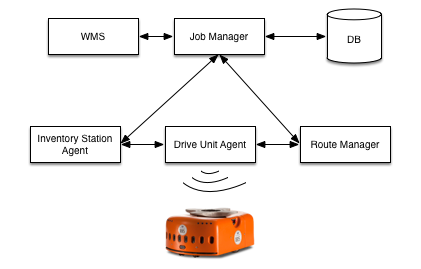
\includegraphics[width=.8\textwidth]{images/Amazon.png}
        \caption{Amazon multi-agent architecture. \tiny{Original in \cite{Wurman2014}}.}
\end{figure}

	
\end{columns}

\end{frame}

%------------------------------------------------
\section*{}

\begin{frame}
\frametitle{References}
\footnotesize{
\begin{thebibliography}{99} % Beamer does not support BibTeX so references must be inserted manually as below
\bibitem[Fazlollahtabar et al., 2015]{Fazlollahtabar2015} Fazlollahtabar et al. (2015)
%\bibitem{Fazlollahtabar2015}
\newblock Autonomous Guided Vehicles
\newblock \emph{Springer-Verlag}

\bibitem[Oleari et tal., 2014]{Oleari2014} Oleari et tal. (2014)
\newblock Industrial AGVs: Toward a pervasive diffusion in modern factory warehouses
\newblock \emph{Proceedings - 2014 IEEE 10th International Conference on Intelligent Computer Communication and Processing, ICCP 2014}

\bibitem[Wurman, 2014]{Wurman2014}
Wurman, P. R. (2014), 
\newblock “How to Coordinate a Thousand Robots,” 
\newblock \emph{International Conference on Automated Planning and Scheduling (ICAPS), 2014}

\end{thebibliography}
}
\end{frame}


\end{document}